\chapter{Hardware Design}
The General hardware design is explained using following the hierarchy graph.

\begin{figure}[H]
    \centering
    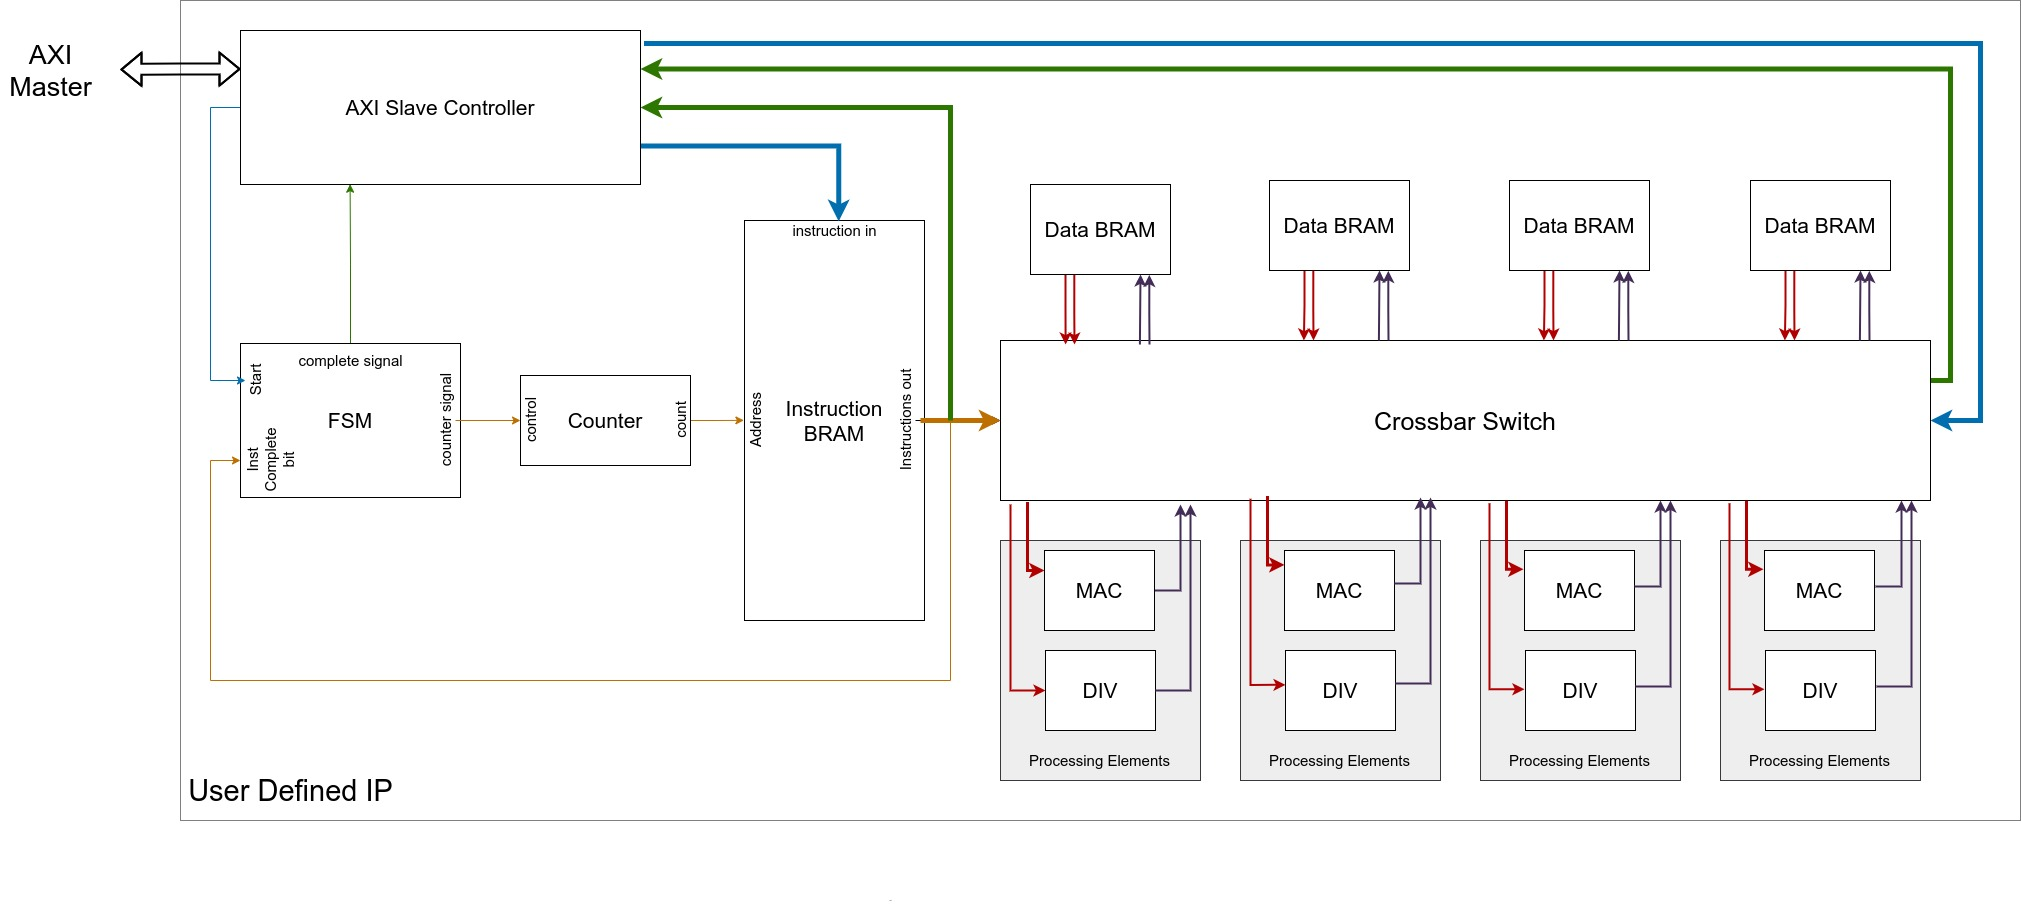
\includegraphics[width = \textwidth]{./Hardware/OWN_Hardware.jpg}
    \caption{Hardware architecture}
    \label{fig:sym:flowGraph}
\end{figure}


The design uses Xilinx optimized IP, and a Crossbar switch box is used to interconnect the overall design as per the requirement for the accelerator. Following are the IPs used:-
\begin{itemize}
	\item Block Memory Generator (BRAM Unit) \cite{Xilinx_BRAM}
		\begin{itemize}
		\item Instruction BRAM (custom bit size)
		\item Data BRAM (float / double type)
		\end{itemize}
	\item Floating-point \cite{Xilinx_Floatpt}
		\begin{itemize}
			\item Fused Multiply-Add/Sub (MAC Unit)
			\item Division (DIV Unit)
		\end{itemize}
\end{itemize}

\section{Block Memory Generator (BRAM Unit) IP}

The Xilinx LogiCORE IP Block Memory Generator replaces the Dual Port Block Memory and Single Port Block Memory LogiCOREs but is not a direct drop-in replacement. It should be used in all new Xilinx designs. The core supports RAM and ROM functions over a wide range of widths and depths. Use this core to generate block memories with symmetric or asymmetric read and write port widths and centers that can perform simultaneous write operations to separate locations and simultaneous read operations from the exact location. For more information on differences in interface and feature support between this core and the Dual Port Block Memory and Single Port Block Memory LogiCOREs, please consult the datasheet.
\\
\\
The BRAM Units are used for instructions produced by the scheduler and storing $A$ and $LU$ Matrix values. The instructions BRAM used to select change the connection of crossbar switch in the design, which would lead to floating-point operations as per the schedule for Decomposition. The instructions BRAM is custom input/output bit as per the scheduler, and Data BRAM should be 32bit / 64bit as per the data type.

\section{Floating-point IP}
The Xilinx Floating-Point Operator is capable of being configured to provide a range of floating-point operations. The core offers addition, subtraction, accumulation, multiplication, fused multiply-add, division, reciprocal, square-root, reciprocal-square-root, absolute value, logarithm, exponential, compare, and conversion operations. High-speed, single-cycle throughput is provided at a wide range of word lengths, including half, single and double precision. DSP48 slices can be used with specific operations.
\\
\\
The floating-point IP is used to Multiply and Accumulate Unit and Divider Unit.
\\
\\
The LU factorization requires only a floating-point multiplier and subtract operation ($Result = C - AB$).The Xilinx's MAC units utilize on-chip DSP Slices to achieve higher performance.
\\
\\
The Xilinx Floating Point Divider IP utilizes some radix-2 SRT division algorithm variants and can not use DSP slices. These units are bulkier and therefore have to be deeply pipelined to operate. The speed grade of the target FPGA is one of the most dominating factors in determining the depth of the pipeline.


\section{Crossbar switch box}

The Crossbar switch box should connect any output port to an input port for  Data BRAMs, MAC, and DIV units. This can be achieved with a multiplexer. The select signals are provided by instructions BRAMs, which were produced by the scheduler. The number of multiplexers depends on Processing elements, the Number of Data BRAMs, and the number of ports at each BRAM.
\\
\\
The top-level design is developed into IP via AXI slave wrapper to connect soft-core and/or hard-core processors. The Crossbar switch box should instruct BRAM and Data BRAM to upload data/instruction and receive Matrix Decomposed Matrix.
\pagebreak